\chapter{Anexos}

\section{Pantallas básicas del Núcleo}


\begin{figure}[!htbp]
  \centering
    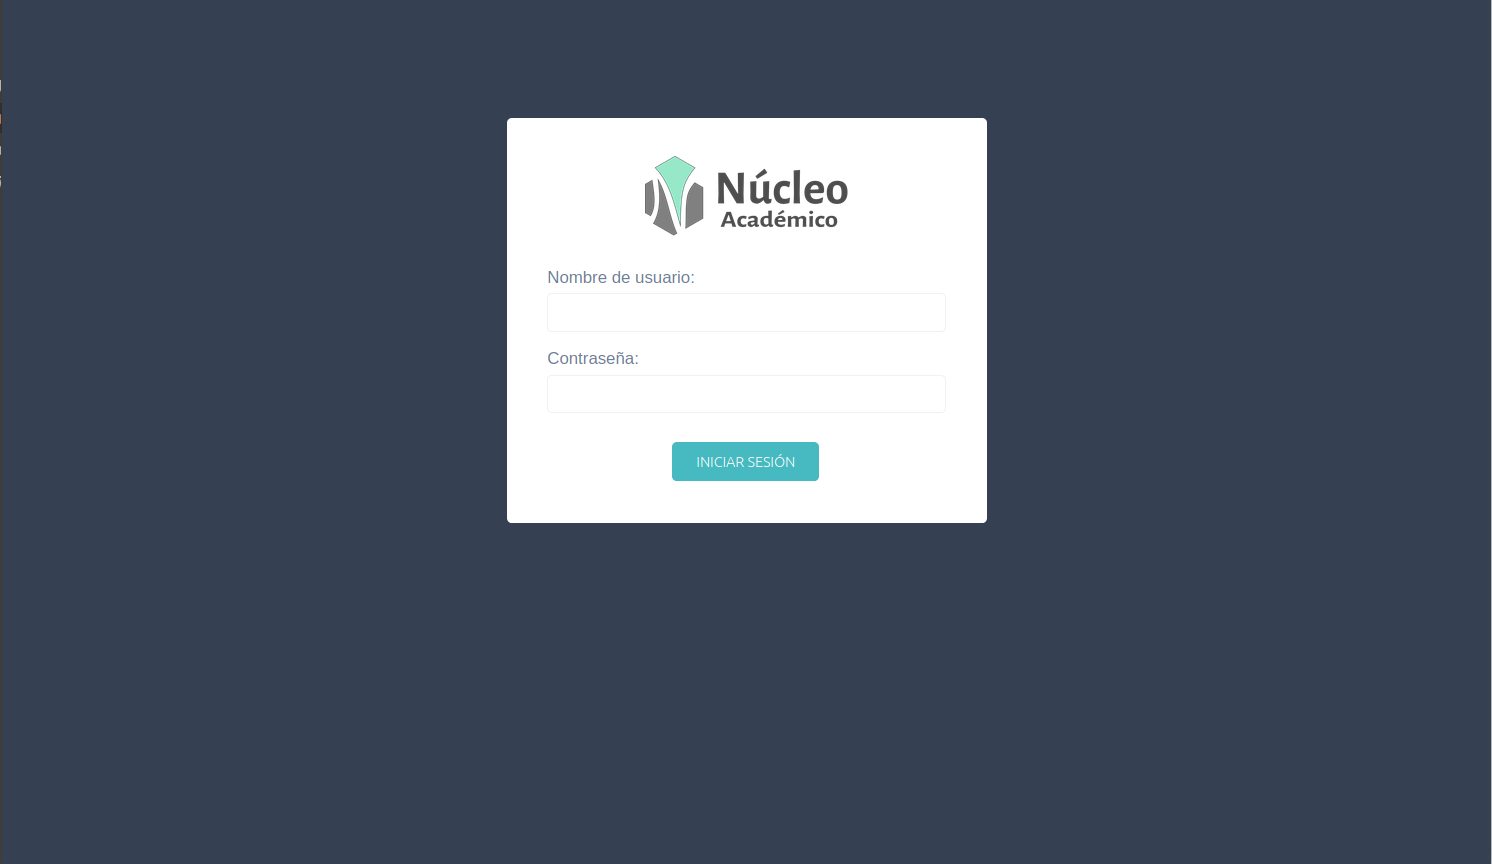
\includegraphics[scale=0.3]{images/nucleo/nucleo-login.png}
  \captionof{figure}{Pantalla de login}
  \label{fig:nucleo-login}
\end{figure}

\begin{figure}[!htbp]
  \centering
    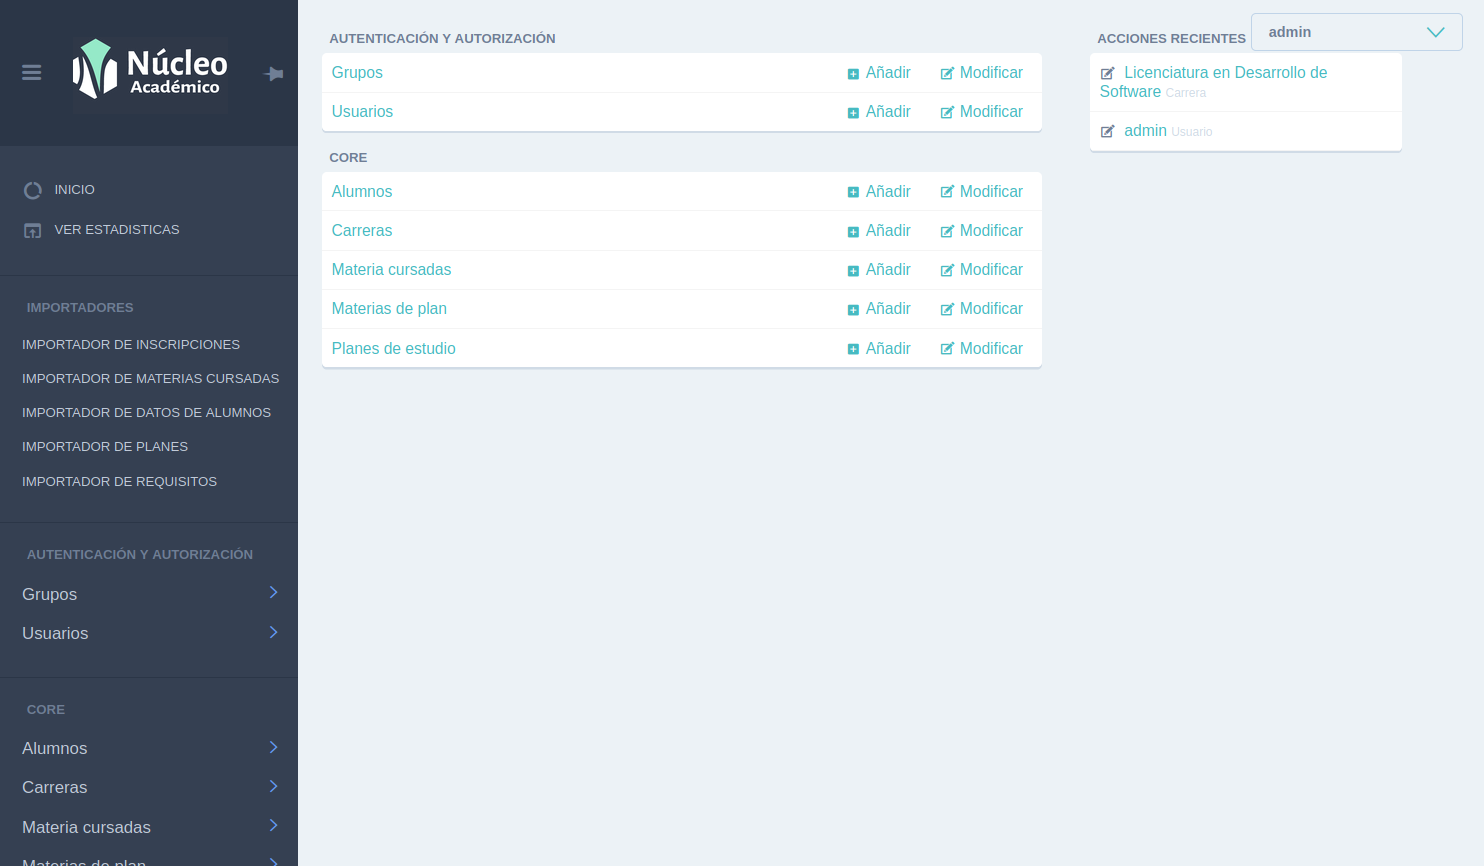
\includegraphics[scale=0.3]{images/nucleo/nucleo-home.png}
  \captionof{figure}{Pantalla principal del admin}
  \label{fig:nucleo-home}
\end{figure}

\begin{figure}[!htbp]
  \centering
    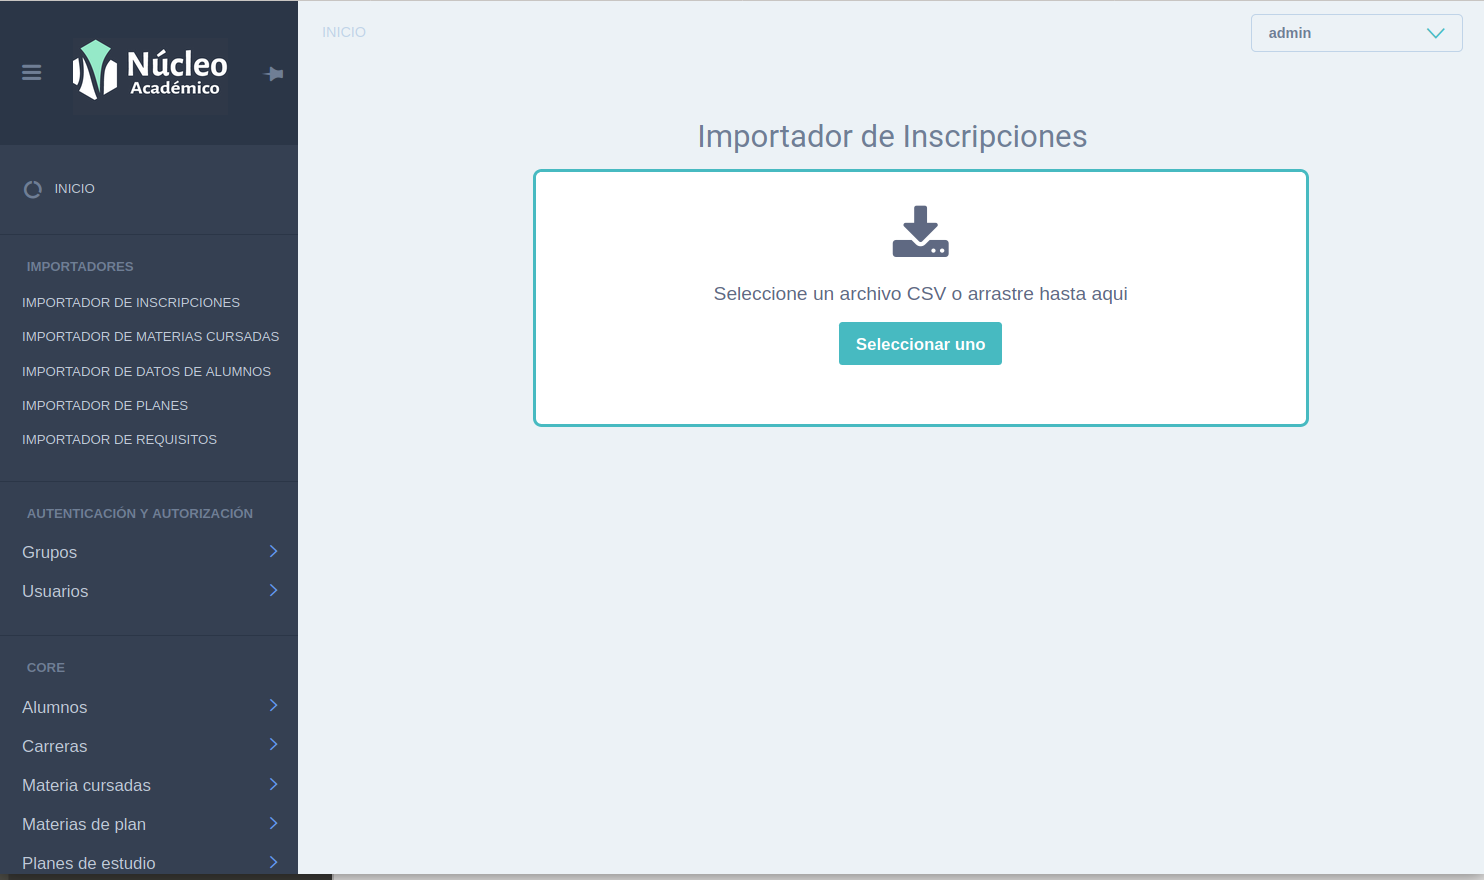
\includegraphics[scale=0.3]{images/nucleo/nucleo-importador.png}
  \captionof{figure}{Pantalla de importadores}
  \label{fig:nucleo-importador}
\end{figure}

\begin{figure}[!htbp]
  \centering
    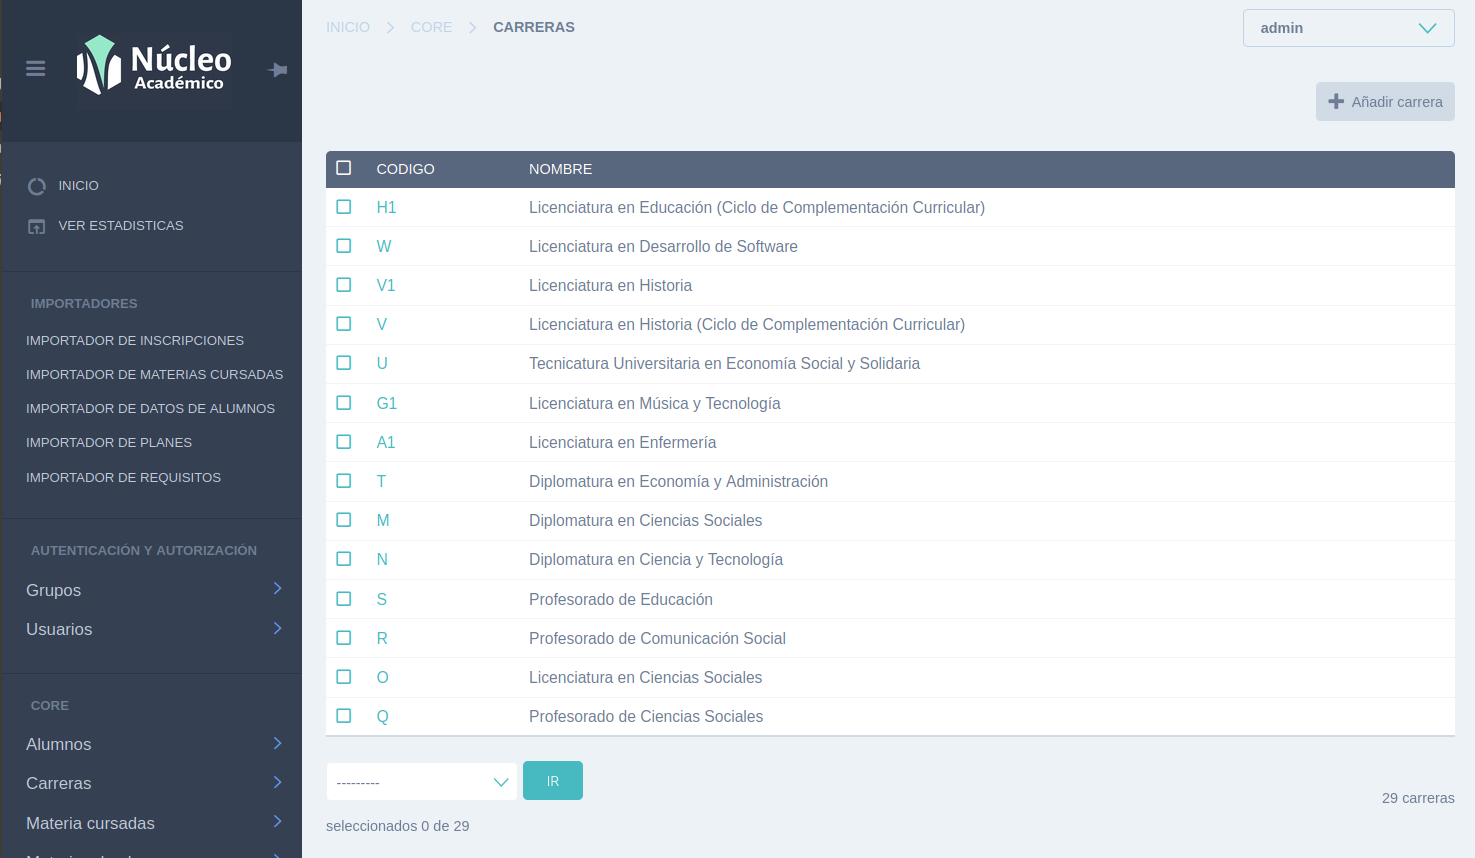
\includegraphics[scale=0.3]{images/nucleo/nucleo-list.png}
  \captionof{figure}{Pantalla de listados}
  \label{fig:nucleo-listado}
\end{figure}

\begin{figure}[!htbp]
  \centering
    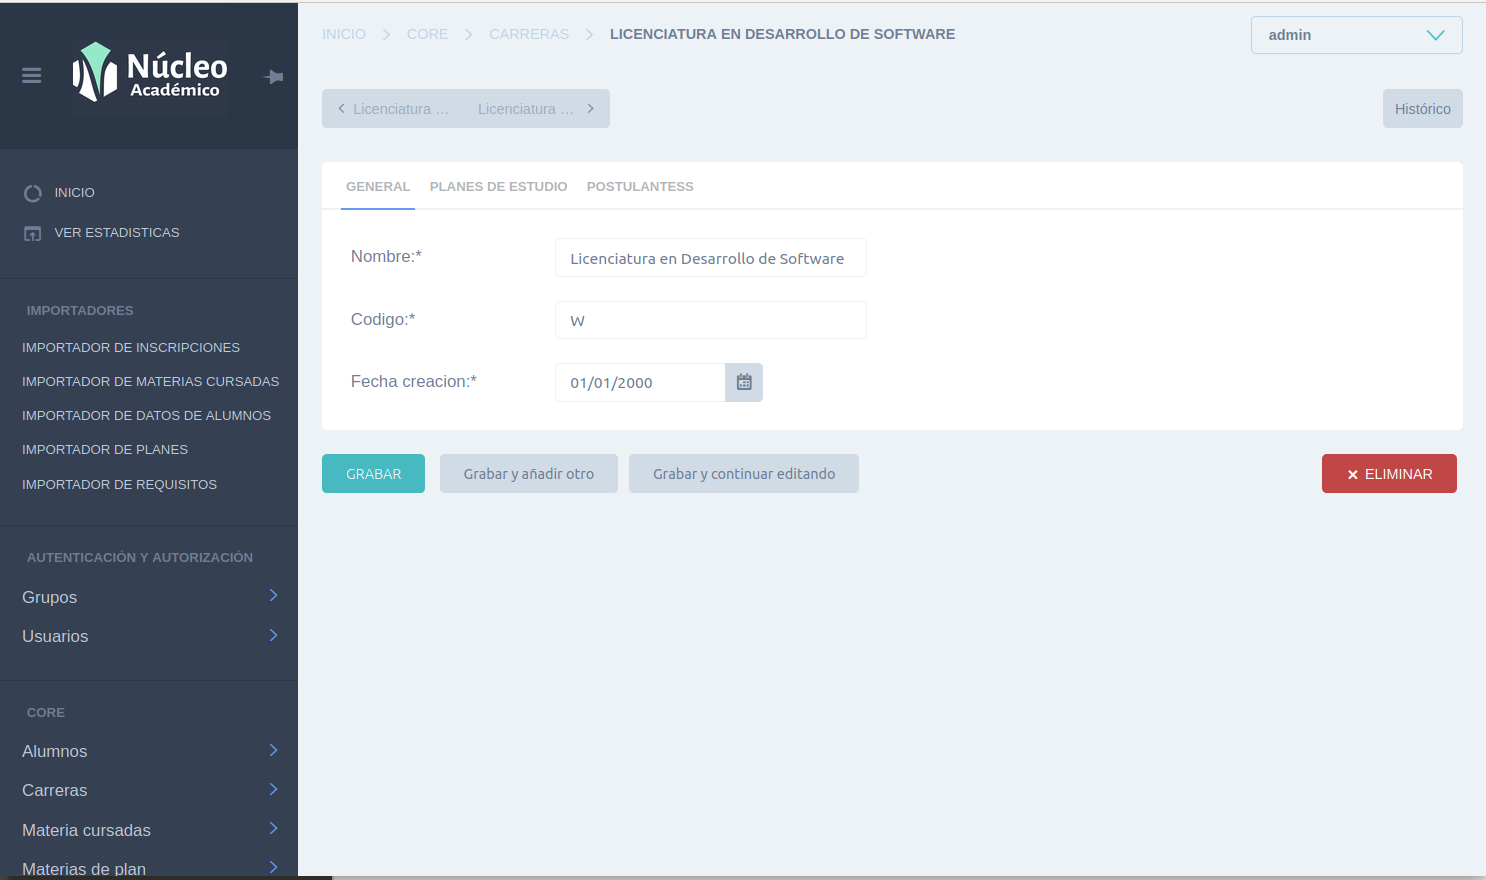
\includegraphics[scale=0.3]{images/nucleo/nucleo-edit.png}
  \captionof{figure}{Pantalla de edición}
  \label{fig:nucleo-edicion}
\end{figure}

\begin{table}[!htbp]
    \centering
    \makegapedcells
    \begin{tabular}{|c|c|c|c|c|}
    \hline
    URI & Método & Parámetros & Content-Type \\ \hline
    api/token/ & POST & username,password & application/x-www-form-urlencoded \\ \hline
    \end{tabular}
    \caption{Método para pedir un token al núcleo}
    \label{tab:tabla_token}
\end{table}

\begin{table}[!htbp]
    \centering
    \makegapedcells
    \begin{tabular}{|c|c|c|}
    \hline
    URI & Método & Autorización\\ \hline
    carreras/<str:cc>/alumnos/ & GET & Bearer  \\ \hline
    carreras/<str:cc>/alumnos-completos/ & GET & Bearer  \\ \hline
    carreras/<str:cc>/planes/<int:plan\_anio>/ & GET & Bearer  \\ \hline
    carreras/<str:cc>/planes/<int:pa>/cantidad-materias-necesarias/ & GET & Bearer  \\ \hline
    carreras/<str:cc>/planes/ & GET & Bearer  \\ \hline
    carreras/<str:cc>/materiascursadas/ & GET & Bearer  \\ \hline
    carreras/<str:cc>/inscripciones/ & GET & Bearer  \\ \hline
    carreras/<str:cc>/cantidad-graduados/ & GET & Bearer  \\ \hline
    carreras/<str:cc>/cantidad-graduados/<int:anio>/ & GET & Bearer  \\ \hline
    carreras/<str:cc>/cantidad-cursantes/ & GET & Bearer  \\ \hline
    carreras/<str:cc>/cantidad-cursantes/<int:anio>/ & GET & Bearer  \\ \hline
    carreras/<str:cc>/cantidad-ingresantes/ & GET & Bearer  \\ \hline
    carreras/<str:cc>/cantidad-ingresantes/<int:anio>/ & GET & Bearer  \\ \hline
    carreras/<str:cc>/cantidad-postulantes/<int:anio>/ & GET & Bearer  \\ \hline
    carreras/<str:cc>/cantidad-postulantes/ & GET & Bearer  \\ \hline
    alumno/<str:legajo>/cursadas/ & GET & Bearer  \\ \hline
    alumno/<str:legajo>/inscripciones/ & GET & Bearer  \\ \hline
    materia/<str:codigo>/alumnos/ & GET & Bearer  \\ \hline
    \end{tabular}
    \caption{Métodos para pedir datos. (cc: código de carrera, pa: plan año)}
    \label{tab:tabla_api}
\end{table}

\section{Pantallas básicas de Seguimiento Académico}

\begin{figure}[!htbp]
  \centering
    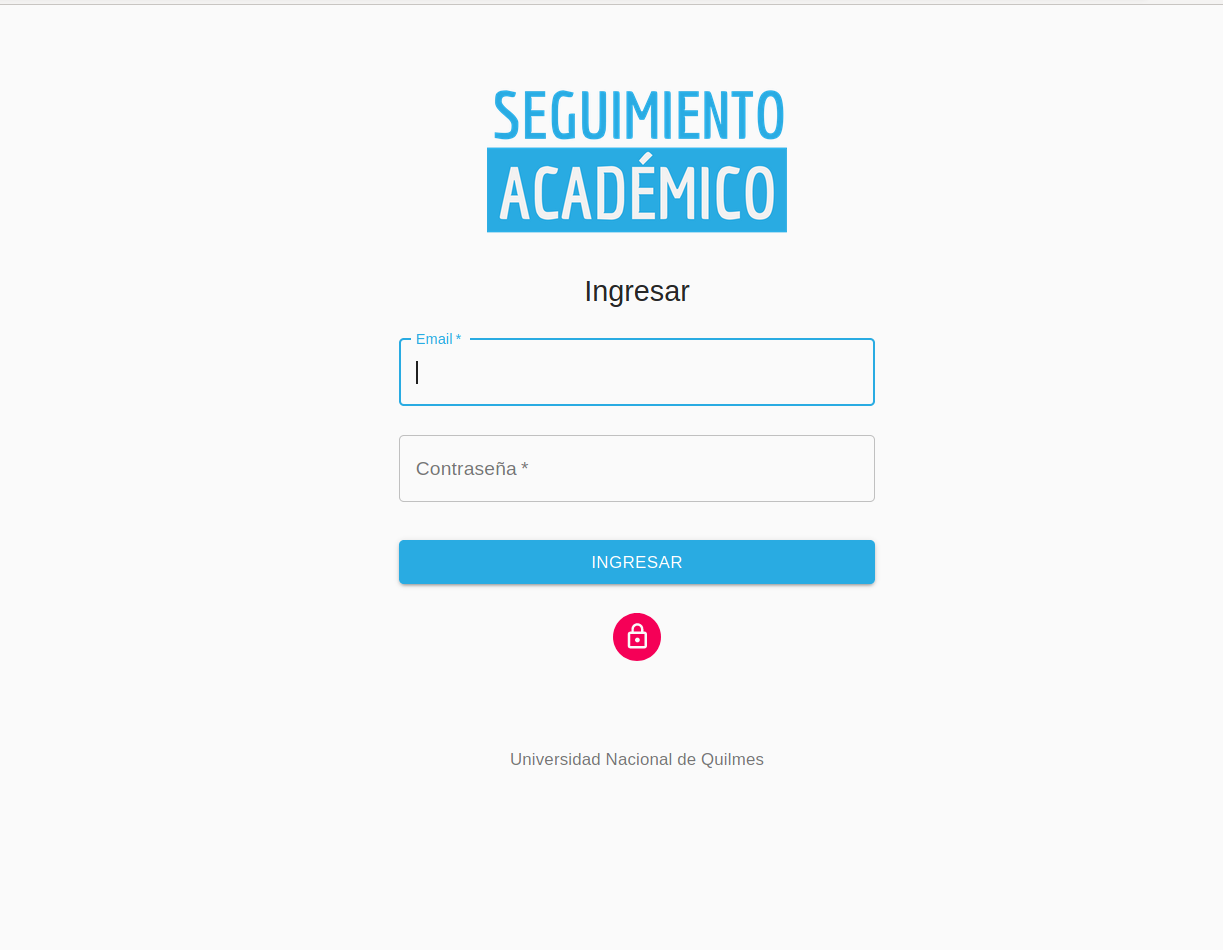
\includegraphics[scale=0.3]{images/seguimiento-academico/sa-login.png}
  \captionof{figure}{Login de Seguimiento Académico}
  \label{fig:sa-login}
\end{figure}

\begin{figure}[!htbp]
  \centering
    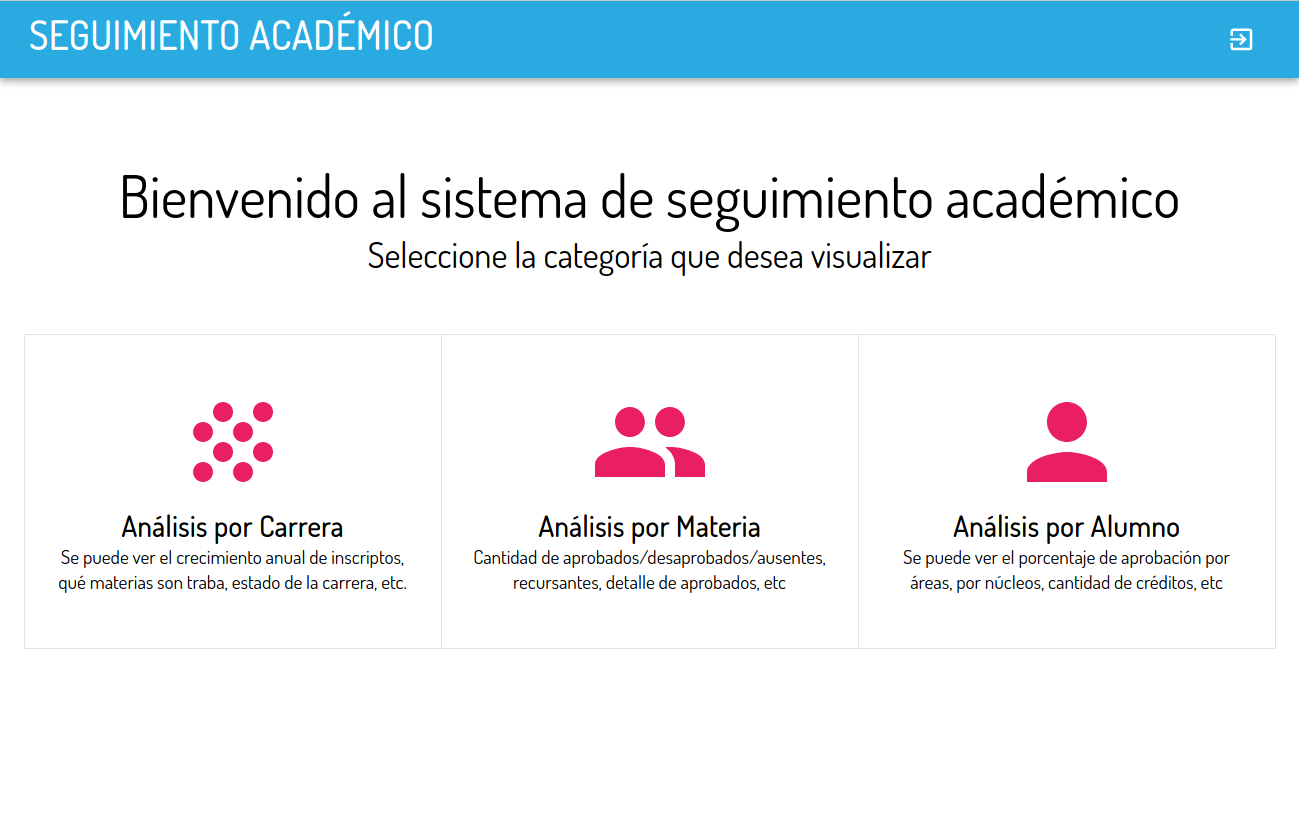
\includegraphics[scale=0.3]{images/seguimiento-academico/sa-home.png}
  \captionof{figure}{Pantalla principal de Seguimiento Académico}
  \label{fig:sa-home}
\end{figure}

\begin{figure}[!htbp]
  \centering
    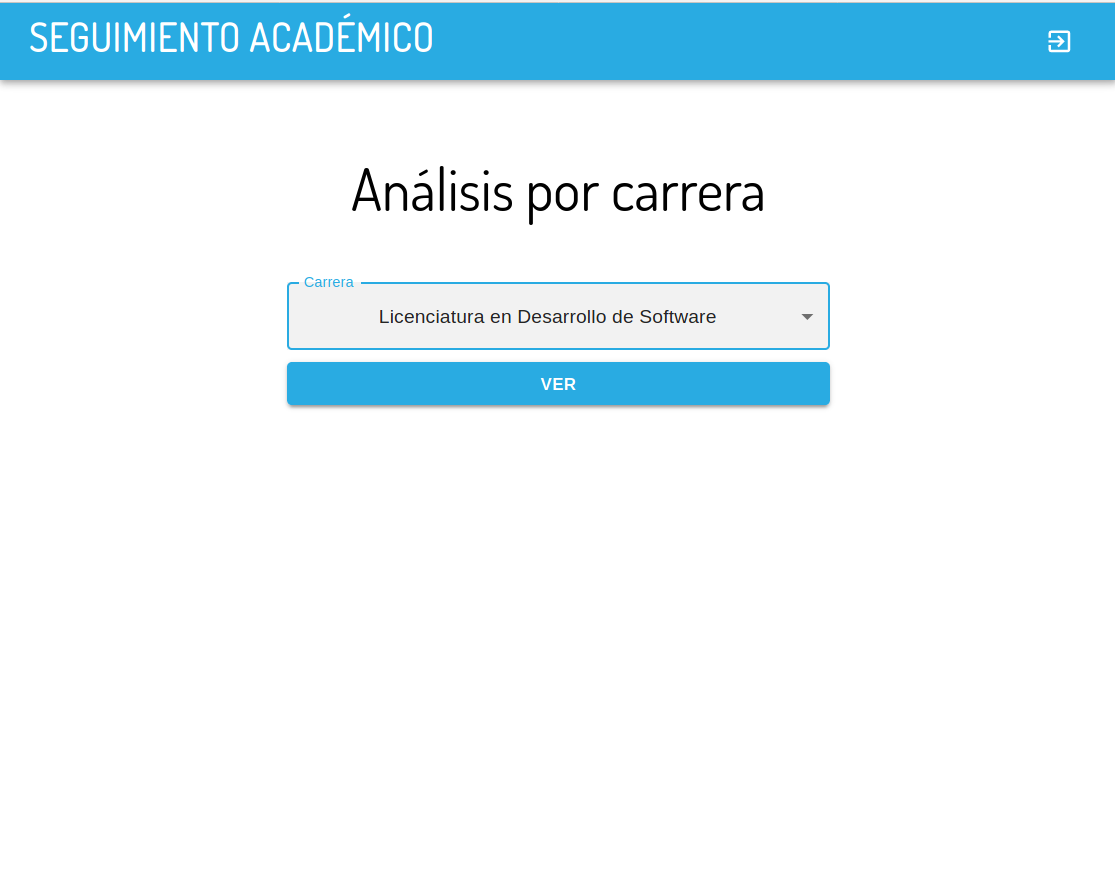
\includegraphics[scale=0.3]{images/seguimiento-academico/sa-form-carrera.png}
  \captionof{figure}{Pantalla Reporte de Carrera de Seguimiento Académico}
  \label{fig:sa-carrera}
\end{figure}

\begin{figure}[!htbp]
  \centering
    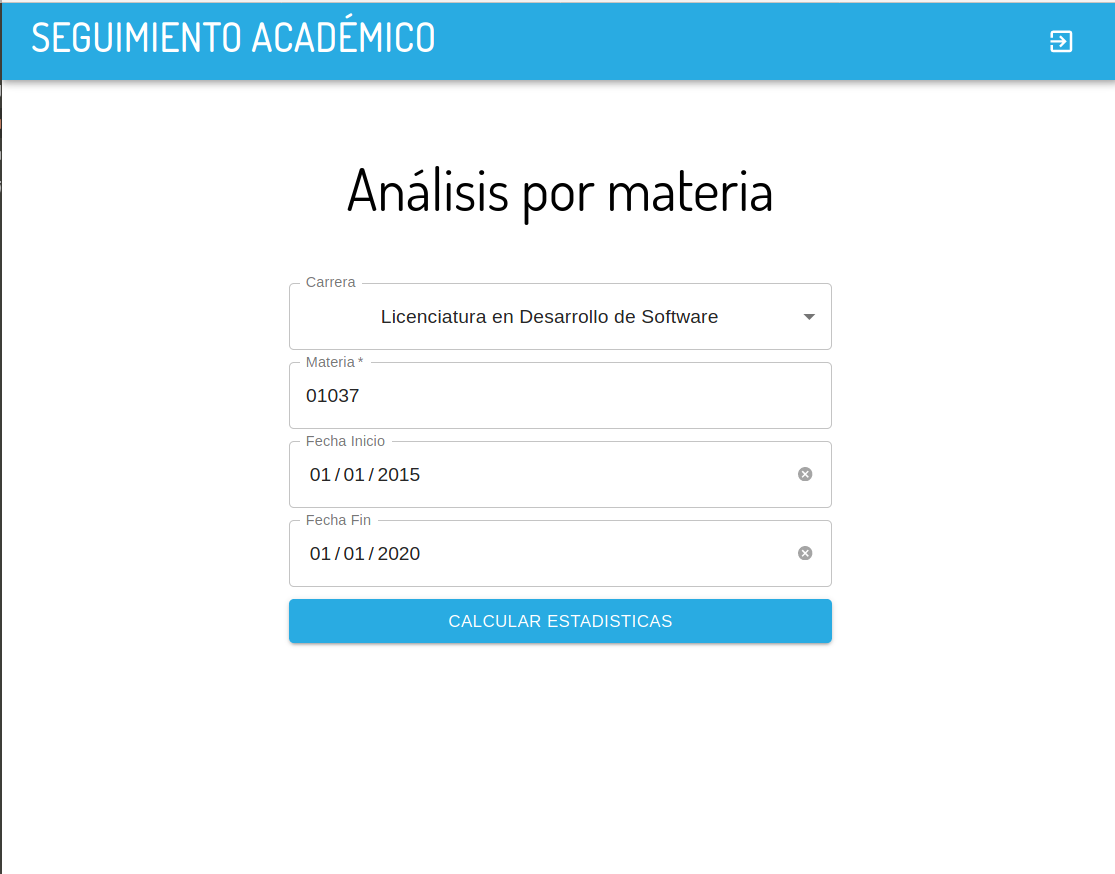
\includegraphics[scale=0.3]{images/seguimiento-academico/sa-form-materia.png}
  \captionof{figure}{Pantalla Reporte de Materia de Seguimiento Académico}
  \label{fig:sa-materia}
\end{figure}

\begin{figure}[!htbp]
  \centering
    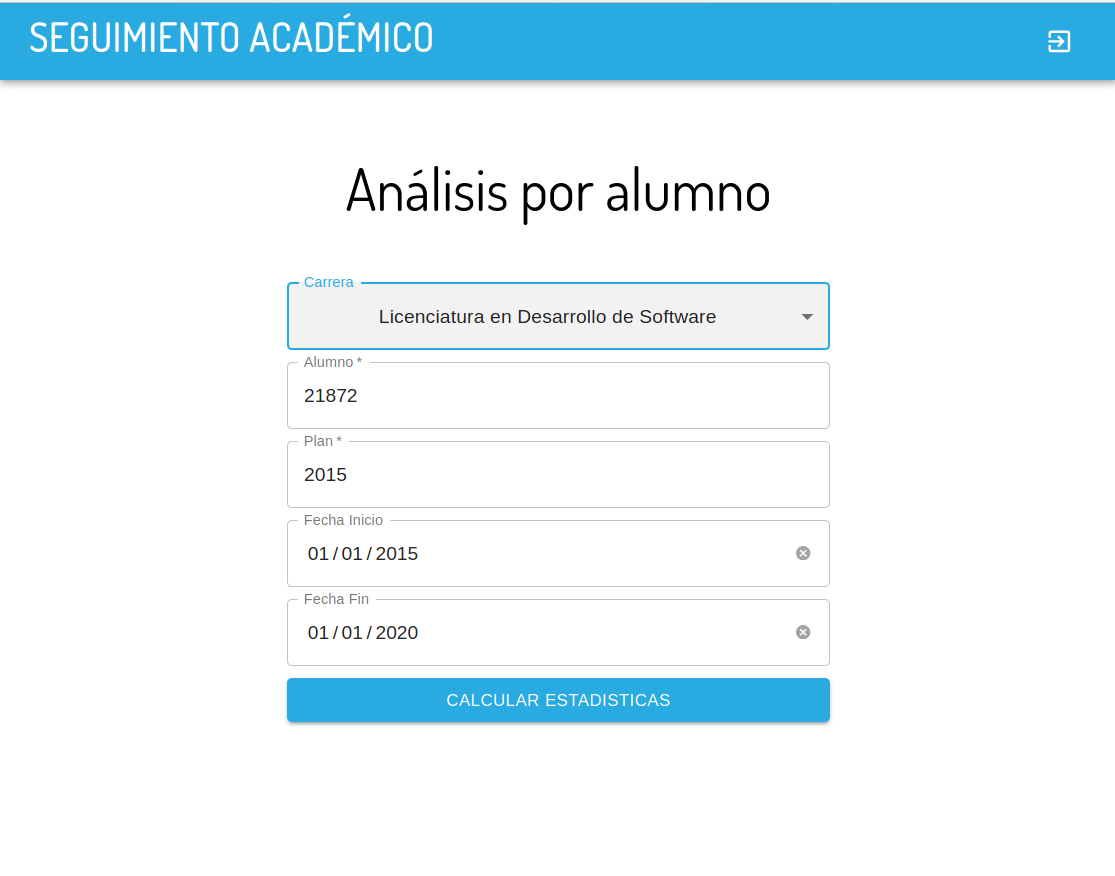
\includegraphics[scale=0.3]{images/seguimiento-academico/sa-form-alumno.png}
  \captionof{figure}{Pantalla Reporte de Alumno de Seguimiento Académico}
  \label{fig:sa-alumno}
\end{figure}


\section{Pantallas básicas de Seguimiento Académico versión Móvil}

\begin{figure}[!htbp]
  \centering
    
\includegraphics[scale=0.3]{images/seguimiento-academico/sa-mobile-login.png}
  \captionof{figure}{Login de Seguimiento Académico Versión móvil}
  \label{fig:sa-login-mobile}
\end{figure}

\begin{figure}[!htbp]
  \centering
    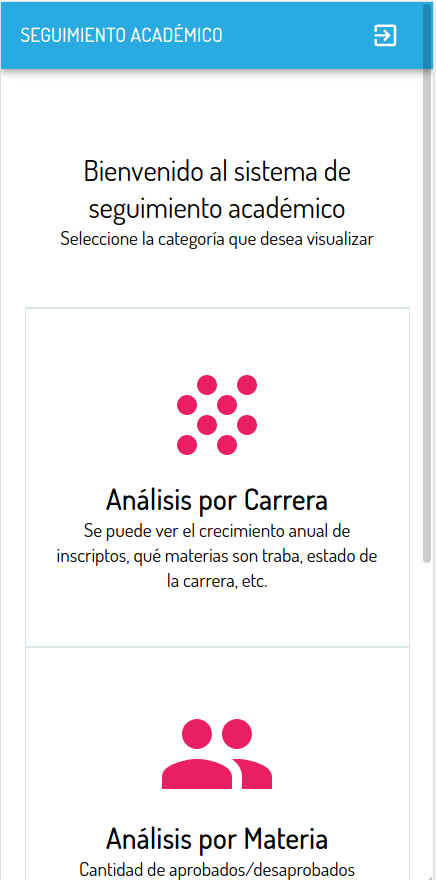
\includegraphics[scale=0.3]{images/seguimiento-academico/sa-mobile-home.png}
  \captionof{figure}{Pantalla principal de Seguimiento Académico versión móvil}
  \label{fig:sa-home-mobile}
\end{figure}

\begin{figure}[!htbp]
  \centering
    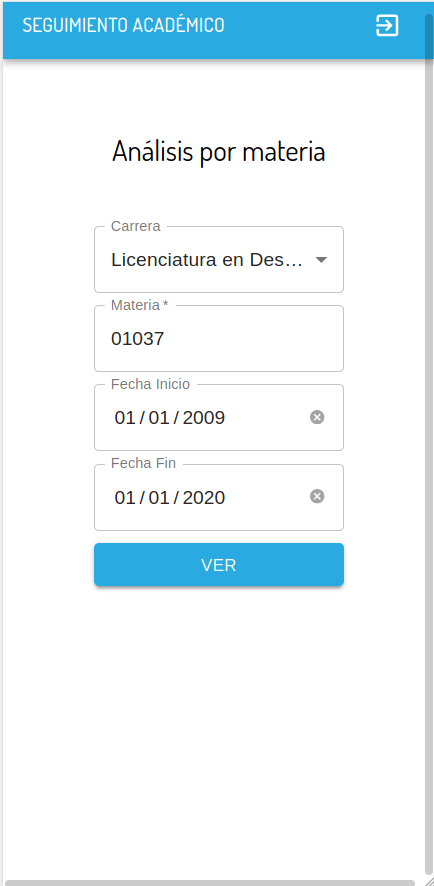
\includegraphics[scale=0.3]{images/seguimiento-academico/sa-mobile-materias-form.png}
  \captionof{figure}{Pantalla Reporte de Materia de Seguimiento Académico versión móvil}
  \label{fig:sa-materia-form-mobile}
\end{figure}

\begin{figure}[!htbp]
  \centering
    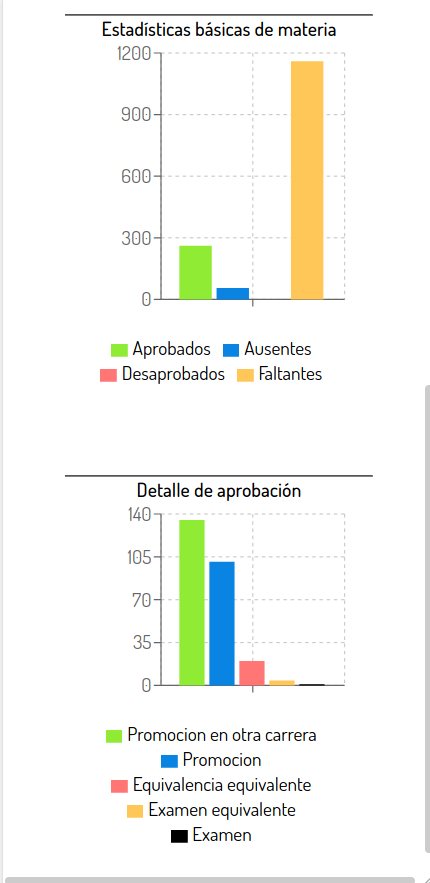
\includegraphics[scale=0.3]{images/seguimiento-academico/sa-mobile-materias.png}
  \captionof{figure}{Pantalla Reporte de Materia de Seguimiento Académico versión móvil}
  \label{fig:sa-materia-mobile}
\end{figure}